

The PAK/PPK protocols were first introduced by Boyko, MacKenzie and Patel in~\cite{BoMaPa00} in 2000
as Diffie-Hellman based provably secure PAKEs, with the PAK protocol admitting key confirmation
and PPK admitting only key authentication (although PPK) uses one less round of communication). 
An augmented variant of PAK, called PAK-X, was also introduced in the same paper.

%The setting of PAK/PPK is similar to all other Diffie-Hellman based PAKEs. What is different is its dependencies on perfect hash functions.

Let $\pi$ be the password shared by Alice and Bob and $p$ and $q$ be primes with $p = rq+1$, where $q \not | r$.
Furthermore, let $g$ be a generator of a subgroup of $\mathbb{Z}^\ast_p$ of size $q$ where the Decision
Diffie-Hellman (DDH) problem is infeasible. Finally, we take $H_1, H_{2a}, H_{2b}, H_3$ to be independent random hash 
functions. The PAK and PPK protocols are described as in Figures \ref{fig:pak} and \ref{fig:ppk}. 
\comment{Re-do diagrams for ourselves}

\begin{figure}[h]
    \centering
    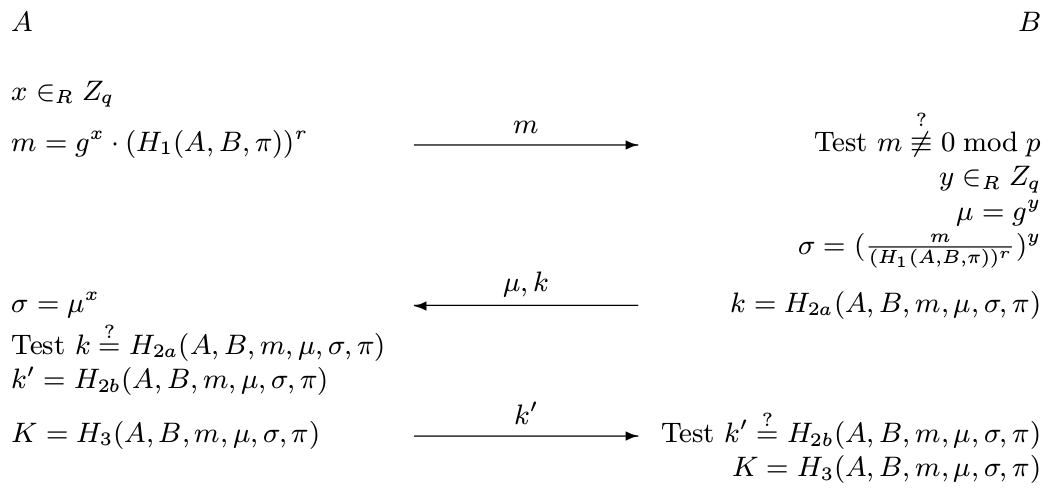
\includegraphics[scale=0.4]{pak_protocol.png}
    \caption{The PAK protocol.}
    \label{fig:pak}
\end{figure}

\begin{figure}[h]
    \centering
    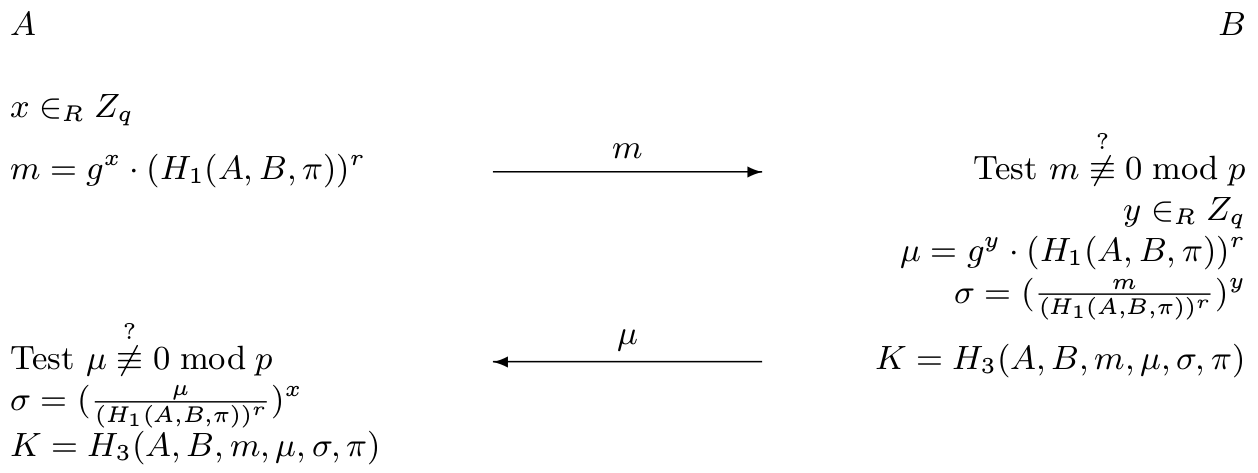
\includegraphics[scale=0.33]{ppk_protocol.png}
    \caption{The PPK protocol.}
    \label{fig:ppk}
\end{figure}

In their original paper, Boyko, MacKenzie and Patel~\cite{BoMaPa00} developed a new formal model for PAKE
security, in which they proved that PAK and PPK are secure under the assumptions of the random-oracle model and
the hardness of the DDH is intractable. This newly proposed model was well designed, and security proofs of other
PAKE protocols have been tailored to it (for instance, the security proof of SPEKE given by MacKenzie\cite{Mac01} 
and mentioned in Section~\ref{sec:SPEKE}).












